\section{Objetivos}

Entre otras caracter�sticas, el principal objetivo de MIEX es analizar
sint�cticamente colecciones de peque�os documentos escritos en ingl�s. En el
siguiente cap�tulo se ver� con m�s profundidad el funcionamiento interno, pero
si por ahora nos abstraemos, lo primero deber�a de ser separar cada documento
en oraciones y posteriormente analizarlas.

Se realizan dos tipos de an�lisis, a nivel de palabra individual, y a nivel de
relaciones entre palabras, vamos a ver un ejemplo. Veamos que an�lisis produce
el analizador para la siguiente oraci�n.

\textit{The Debian Project is an association of individuals.}

La representaci�n m�s vistosa del resultado es en forma de �rbol, por lo que lo
dibujaremos as�. Para saber el significado de cada etiqueta no tiene m�s que
echar un vistazo al anexo \ref{sec:penntags}.

\Tree[.ROOT [.S [.NP [.DT The ] [.NNP Debian ] [.NNP Project ] ] [.VP [.VBZ is
] [.NP [.NP [.DT an ] [.NN association ] ] [.PP [.IN of ] [.NP [.NNS individuals
 ] ] ] ] ] ] ]
 

Se puede ver que se asignan etiquetas a nivel de palabra, a nivel de grupo
frasal y a nivel clausal, tal y como se hace habitualmente en cualquier an�lisis
sint�ctico.

Aprovecharemos tambi�n que el analizador calcula las dependencias entre algunas
palabras de la oraci�n:

\begin{Verbatim}[fontsize=\relsize{-1}]
det(Project-3, The-1)
nn(Project-3, Debian-2)
nsubj(association-6, Project-3)
cop(association-6, is-4)
det(association-6, an-5)
prep_of(association-6, individuals-8)
\end{Verbatim}

Tanto el an�lisis a nivel de palabra (y obviamente a nivel de grupo) como las
relaciones entre las palabras ser� la informaci�n que nos va a interesar
guardar.

En resumen, una buena visi�n global de los objetivos de MIEX es la siguientes:

\begin{itemize}
	\item Comprobaci�n de integridad y an�lisis de documentos XML.
	\item Uso del Stanford Parser para extraer los an�lisis
sint�cticos de las oraciones as� como las relaciones entre las palabras.
	\item An�lisis y limpieza de la informaci�n recabada.
	\item Almacenamiento en un medio flexible para posteriormente realizar
consultas a medida.
\end{itemize}


\begin{figure}[h]
\begin{center}
	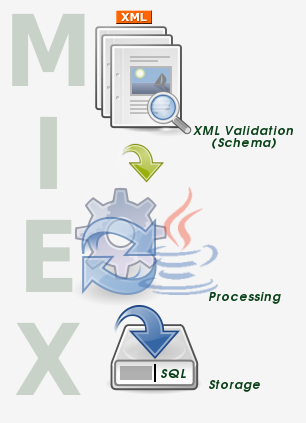
\includegraphics[bb=0 0 148 240]{images/miex.png}
	% miex.png: 257x416 pixel, 125dpi, 5.22x8.45 cm, bb=0 0 148 240
\end{center}
\caption{Diagrama simplificado de funcionamiento}
\end{figure} 
